\documentclass{jacsart}
\usepackage{hyperref}
\usepackage{cite}
\usepackage{stfloats}
\usepackage{url}
\usepackage{authblk}
\usepackage[utf8]{inputenc}
\usepackage[T1]{fontenc}
\usepackage{graphicx}
\usepackage{amsthm}
\usepackage{txfonts}
\usepackage[textsize=tiny]{todonotes}

\newtheorem{definition}{Definition}
\newtheorem{theorem}[definition]{Theorem}
\newtheorem{corollary}[definition]{Corollary}
\newtheorem{proposition}[definition]{Proposition}
\newtheorem{example}[definition]{Example}


\providecommand{\tightlist} { \setlength{\itemsep}{0pt}\setlength{\parskip}{0pt}}
\providecommand{\keywords}[1]{ \small	 \textbf{\textit{Keywords---}} #1 }

\title{Object-Oriented Internet - Azure Interoperability}
% \title{Object-Oriented Internet - reactive visualization of asynchronous data using AZURE}
\headtitle{OOI - Azure Interoperability}

\author{Mariusz Postół\inst{1}, Piotr Szymczak\inst{1}, Clemens Vasters\inst{2}}
\headauthor{Postół M, Szymczak P, Vasters C}
\affiliation{%
 \inst{1}Lodz University of Technology\\
 Institute of Information Technology\\
 ul. Wólczańska 215, 90-924 Lodz, Poland\\
 mailto:mariusz.postol@p.lodz.pl
 \andinst
 \inst{2}Microsoft\\
 Faculty/Department/Office Name\\
 Postal Address with the zip-code\\
 clemensv@microsoft.com}

\keywords{Azure, Cloud Computing, Object-Oriented Internet, Industrial communication, Industry 4.0, Internet of Things, Machine to Machine Communication, OPC Unified Architecture}

\begin{document}

\maketitle


\begin{abstract}

  Lorem ipsum dolor sit amet, consectetur adipiscing elit. Sed luctus neque eu erat pulvinar rutrum. Sed id congue leo. Pellentesque ornare enim libero, convallis eleifend turpis rhoncus ac. Proin eget pellentesque dolor. Phasellus lacinia velit eget faucibus iaculis. Pellentesque consequat erat non urna scelerisque cursus. Donec urna nisi, pulvinar a nisl eu, lobortis sollicitudin nulla. Proin tempus risus vel lacinia vestibulum. Praesent eget nisi lorem. Nam rutrum lectus vulputate dolor venenatis eleifend. Sed dolor lacus, cursus non enim tincidunt, auctor hendrerit orci. Donec venenatis ultrices est, nec molestie lorem. Morbi eleifend mattis ex, eget mollis leo blandit ut. Nulla sed felis posuere, gravida dui sed, iaculis neque. Donec ante purus, rhoncus eu neque tristique, pretium elementum purus.

  Sed euismod maximus consequat. Pellentesque nec leo ligula. Aenean id lorem ac nisi blandit ultrices sit amet nec velit. Vestibulum bibendum ipsum vulputate quam suscipit, eu tincidunt diam imperdiet. Nunc vel turpis ut tortor bibendum ullamcorper sed ut magna. Sed sit amet quam ut lacus pretium ullamcorper. Fusce feugiat ornare mollis. Vestibulum sagittis velit id augue tempus, in vestibulum velit bibendum. Curabitur ac aliquet mi. Aliquam erat volutpat. Cras quis dignissim est, ac gravida.
\end{abstract}

\maketitle

\listoftodos[TODO list]

\hypertarget{introduction}{%
  \section{Introduction}\label{introduction}}

All the time, the Information and Communication Technology is providing
society with a vast variety of new distributed applications aimed at
micro and macro optimization of the industrial processes. Obviously, the
design foundation of this kind of application has to focus primarily on
communication technologies. Based on the role humans take while using
these applications they can be grouped as follows:

\begin{itemize}
  \tightlist
  \item
        \textbf{human-centric} - information origin or ultimate information
        destination is an operator,
  \item
        \textbf{machine-centric} - information creation, consumption,
        networking, and processing are achieved entirely without human
        interaction.
\end{itemize}

A typical \textbf{human-centric} approach is a web-service supporting,
for example, a web user interface (UI) to monitor conditions, and manage
millions of devices and their data in a typical cloud-based IoT
approach. It is characteristic that, in this case, any uncertainty and
necessity to make a decision can be relaxed by human interaction.
Coordination of robots behavior in a work-cell (automation islands) is a
\textbf{machine-centric} example. In this case, it is essential that any
human interaction is impractical or even impossible. This
interconnection scenario requires the machine to machine communication
(M2M) demanding multi-vendor devices integration.

From the M2M communication concept, a broader concept of a smart factory
can be derived. In this concept, the mentioned robots are only executive
assets of an integrated supervisory control system responsible for macro
optimization of an industrial process composed into one whole.
Deployment of the smart factory concept requires a hybrid solution and
interconnection of the mentioned above heterogeneous environments. This
approach is called the fourth industrial revolution and coined as
Industry 4.0. It is worth stressing that machines - or more general
assets - interconnection is not enough, and additionally, assets
interoperability has to be expected for the deployment of this concept.
In this case, multi-vendor integration makes communication
standardization especially important, namely it is required that the
payload of the message is standardized to be factored on the gathering
site and consumed on the ultimate destination site.

Highly-distributed solutions used to control real-time process
aggregating islands of automation (e.g.~virtual power plants producing
renewable energy) additionally must leverage public communication
infrastructure, namely the Internet. Internet is a demanding environment
for highly distributed process control applications designed atop the
M2M communication paradigm because

\begin{itemize}
  \tightlist
  \item
        it is a globally shareable environment and can be also used by
        malicious users
  \item
        it offers only non-deterministic communication making integration of
        islands of automation designed against the real-time requirements a
        difficult task
\end{itemize}

Today both obstacles can be overcome, and as examples, we have bank
account remote control and voice over IP in daily use. The first
application must be fine-tuned in the context of data security, and the
second is very sensitive on time relationships. Similar approaches could
be applied to adopt the well known in process control industry concepts:

\begin{itemize}
  \tightlist
  \item
        Human Machine Interface (HNI)
  \item
        Supervisory Control and Data Acquisition (SCADA)
  \item
        Distributed Control Systems (DCS)
\end{itemize}

A detailed examination of these solutions is far beyond the scope of
this article. It is only worth stressing that, by design, all of them
are designed on the foundation of interactive communication. Interactive
communication is based on a data polling foundation. In this case, the
application must follow the interactive behavioral model, because it
actively polls the data source for more information by pulling data from
a sequence that represents the process state in time. The application is
active in the data retrieval process - it controls the pace of the
retrieval by sending the requests at its convenience. Such a polling
pattern is similar to visiting the books shop and checking out a book.
After you are done with the book, you pay another visit to check out
another one. If the book is not available you must wait, but you may
read what you selected. The client/server archetype is well suited for
the mentioned above applications.

After dynamically attaching a new island of automation the control
application (responsible for the data pulling) must be reconfigured for
this interoperability scenario. In other words, in this case, the
interactive relationship cannot be directly applied because the control
application must be informed on how to pull data from a new source. As a
result, a plug and produce scenario cannot be seamlessly applied. A
similar drawback must be overcome if for security reasons suitable
protection methods have been applied to make network traffic propagation
asymmetric. It is accomplished using intermediary devices, for example,
firewalls, to enforce traffic selective availability based on
predetermined security rules against unauthorized access.

Going further, we shall assume that islands of automation are mobile,
e.g.~autonomous cars passing a supervisory controlled service area. In
this case, the behavior of the interconnected assets is particularly
important concerning the environment in which they must interact. This
way we have entered the Internet of Things domain of Internet-based
applications.

If we must bother with the network traffic propagation asymmetry or
mobility of the asset network attachment-points the reactive
relationship could relax the problems encountered while the interactive
approach is applied. In this case, the sessionless publisher-subscriber
communication archetype is a typical pattern to implement the abstract
reactive interoperability paradigm. The sessionless archetype is a
message distribution scenario where senders of messages, called
publishers, do not send them directly to specific receivers, called
subscribers, but instead, categorize the published messages into topics
without knowledge about which subscribers if any, there may be.
Similarly, subscribers express interest in one or more topics and only
receive messages that are of interest, without knowledge about which
publishers, if any, there are. In this scenario, the publishers and
subscribers are loosely coupled.i.e they are decoupled in time, space
and synchronization \cite{RefWorks:doc:5c44e246e4b0591b15ea9e59}.

If the \textbf{machine-centric} interoperability - making up islands of
automation - must be monitored and/or controlled by a supervisory system
cloud computing concept may be recognized as a beneficial solution to
replace or expand the mentioned above applications, i.e.~HMI, SCADA,
DCS, etc. Cloud computing is a method to provide a requested
functionality as a set of services. There are many examples that cloud
computing is useful to reduce costs and increase robustness. It is also
valuable in case the process data must be exposed to many stakeholders.
Following this idea and offering control systems as a service, there is
required a mechanism created on the service concept and supporting
abstraction and virtualization - two main pillars of the cloud computing
paradigm. In the cloud computing concept, virtualization is recognized
as the possibility to share the services by many users, and abstraction
hides implementation details.

Deployment of the hybrid solution providing interoperability of the
\textbf{machine-centric} cyber-physical systems and
\textbf{human-centric} cloud-based front-end can be implemented applying
the following scenarios:

\begin{itemize}
  \tightlist
  \item
        \textbf{direct interconnection} - cloud-based dedicated communication
        services allow to attache it to the cyber-physical system making up a
        consistent M2M communication network using an in-bound protocol stack
  \item
        \textbf{gateway based interconnection} - typical build-in
        communication services allows to attache the cloud computing to the
        cyber-physical system using an out-of-bound protocol stack
\end{itemize}

By design, the direct approach requires that the cloud has to be
compliant with the interoperability standard the cyber-physical system
is built around - it becomes a consistent part of the cyber-physical
system. Data models, roles, and responsibility differences of both
solutions make this approach impractical and imposable to be applied in
typical cases. A more detailed description is covered by the Sect.~\ref*{cloud-to-sensors-field-level-connectivity}.

This article addresses further research on the integration of the
cyber-physical systems in the context of new emerging disciplines,
i.e.~Industry 4.0 (I4.0) and the Internet of Things (IoT). The new
architecture is proposed for integration of the multi-vendor
\textbf{machine-centric} cyber-physical system designed atop of M2M
reactive communication and emerging cloud computing as a
\textbf{human-centric} front-end. To support the multi-vendor
environment OPC Unified Architecture interoperability standard has been
selected. The proposals are backed by proof of concept reference
implementations. Prototyping addresses Microsoft Azure Cloud as an
example. The prototyping outcome has been just published on GitHub as
the open-source (MIT licensed). The proposed solutions have been
harmonized with the more general concept called the Object-Oriented
Internet.

The main goal of this article is to provide proof that:

\begin{enumerate}
  \def\labelenumi{\arabic{enumi}.}
  \tightlist
  \item
        reactive interoperability M2M communication based on the OPC UA
        standard can be implemented as a powerful standalone library without
        dependency on the Client/Server session-oriented archetype
  \item
        Azure interoperability can be implemented as an external part
        employing out-of-band communication without dependency on the OPC UA
        implementation
  \item
        the proposed generic architecture allows that the gateway
        functionality is composable at run-time - no programming required
\end{enumerate}

The remainder of this paper is structured as follows. Sect.~\ref*{cloud-to-sensors-field-level-connectivity} presents the proposed open and reusable software model. It promotes a reactive interoperability pattern and a generic approach to establishing interoperability-context. Sect.~\ref*{azure-main-technology-features} analyzes data presentation user interface, available native communication services, and data/metadata model offered by the Microsoft Azure. The discussion covered by this section is the foundation for selecting services utilized to expose process data and suitable protocol stack to support interconnection. In Sect.~\ref*{ooi-main-technology-features} the discussion focuses on the generic architecture that is to be used as a foundation for further decisions addressing the systematic design of the interoperability of the cyber-physical systems and cloud-based front-end. A reference implementation of this archetype is described in Sect.~\ref*{gateway-implementation}. The most important findings and future work are summarized in Sect.~\ref*{architecture} \todo{overfull}.

\hypertarget{consider-to-add}{%
  \subsection{Consider to add}\label{consider-to-add}}

\hypertarget{scope}{%
  \subsubsection{Scope}\label{scope}}

What we must do to prove the goal have been achieved. Extent or range of
development, view, outlook, application, operation, effectiveness, etc.

\hypertarget{related-work}{%
  \subsubsection{Related work}\label{related-work}}

Any information about available reusable deliverables related to this
work.

\hypertarget{cloud-to-sensors-field-level-connectivity}{%
  \section{Cloud to Sensors Field Level Connectivity}\label{cloud-to-sensors-field-level-connectivity}}

\hypertarget{architecture}{%
  \subsection{Architecture}\label{architecture}}

As it was explained in Sect.~, to follow the Industry 4.0 concept a hybrid environment integrating reactive Machine to Machine interconnection and interactive web-based user interface is required (\ref*{introduction}). The main challenge of the solution in concern is to design a generic but reusable architecture that addresses interoperability of these diverse interconnection scenarios ruled by different requirements, namely

\begin{enumerate}
  \def\labelenumi{\arabic{enumi}.}
  \tightlist
  \item
        \textbf{machine-centric} machine to machine real-time mobile
        interoperability
  \item
        \textbf{human-centric} cloud-based front-end
\end{enumerate}

Interconnection of the reactive \textbf{machine-centric} and interactive \textbf{human-centric} environments can be implemented by applying one of the following scenarios:\todo{overfull}

\begin{itemize}
  \item \textbf{direct interconnection} (tightly coupled scenario) - cloud-based dedicated communication services are engaged to attach it to the cyber-physical system making up a consistent M2M communication network using a common protocol stack
  \item \textbf{gateway based interconnection} (loosely coupled scenario) - native build-in communication services allows attaching the cloud to the cyber-physical system using an out-of-bound protocol stack
\end{itemize}

In the solution in concern, the interconnection of assets is not enough hence their interoperability is expected. In this case, using the same communication stack must be recognized as only a necessary condition. To support interoperability common data understanding is required. By design, the direct approach requires that the cloud has to be compliant
with the interoperability standard the cyber-physical system uses. As a result, it becomes a consistent communication node of the cyber-physical system. Additionally, to meet this requirement the cloud and cyber-physical systems have to establish directly

\begin{itemize}
  \item the same semantic-context
  \item the same security-context
\end{itemize}

The possibility to establish a common semantic-context in the multi-vendor environment makes communication standardization especially important. In this case, it is required that the encoding of the messages payload exchanged over the network (Data Transfer Object - TDO) is standardized so that the payload can be factored on the data-gathering
site and consumed on the ultimate destination data processing sites. Security between the data origin and ultimate data destination refers to the protection of messages (security-context) against malicious users. It is required that communicating parties are using the same cyber-security measures.

The decision to follow the \textbf{direct interconnection} scenario must be derived from an analysis of the capabilities of available services in concern. However, for the development strategy of this type of solutions this analysis can be done partially taking into account two features that can be considered invariable:

\begin{itemize}
  \item by design the cloud-based services must be virtual - they are used to handle many solutions at the same time
  \item by design the M2M communication is usually constrained by the real-time requirements
\end{itemize}

In practice, the set of assets embedded in the cyber-physical system is very stable. On the another hand, the virtualization of services means that they must be very flexible to handle the attachment of new assets proactively (acting in advance) at run time. As a result, by design, the cloud services must be repressible to register and authenticate devices exposing endpoints in the public network to allows the device to access a provisioning cloud service. It requires that a session over the Internet has to be established by the data holding asset at a preparation step.

To meet the requirements of real-time distributed control the cyber-physical system may use protocols applicable only to local computer networks (e.g.~multicast IP, Ethernet, TSN, etc.). Because the cloud services support only protocols handling interconnection over the Internet the interaction with the cloud requires remote agents, i.e.~agents attached locally to the M2M network and implemented by applying one of the following archetypes:

\begin{itemize}
  \item \textbf{edge device} - remote cloud agent acting as an intermediaryfor nodes of the cyber-physical network
  \item \textbf{field level gateway} - a dedicated custom device acting as an intermediary for nodes of the cyber-physical network
  \item \textbf{embedded gateway} - a software part composed into a selected node of the cyber-physical network
\end{itemize}

\textbf{Edge device} is a device that connects directly to the cloud
services but acts as an intermediary for other devices called leaf
devices. Additionally, it allows the selection of initial data
processing and execution of them using local resources. The \textbf{edge
  device} may be located close to the leaf devices and attached to the
cyber-physical network using protocols applicable only to local computer
networks. In this scenario, it is possible to use a custom protocol
stack to get connected to the \textbf{edge device} with the cloud and
helps to save the bandwidth thanks to sending only the results of local
processing. In this approach, the \textbf{edge device} is part of cloud
vendor products and cannot be recognized as a generic solution that can
be used to connect to other clouds at the same time.

The \textbf{field level gateway} is also build atop of the middleware
concept. The only difference compared with the \textbf{edge device} is
necessity to use officially supported by the cloud vendor services to
get connected. In this scenario the process data may be transferred to
many clouds at the same time provided that the gateway offers this
functionality.

\begin{figure}
  \centering
  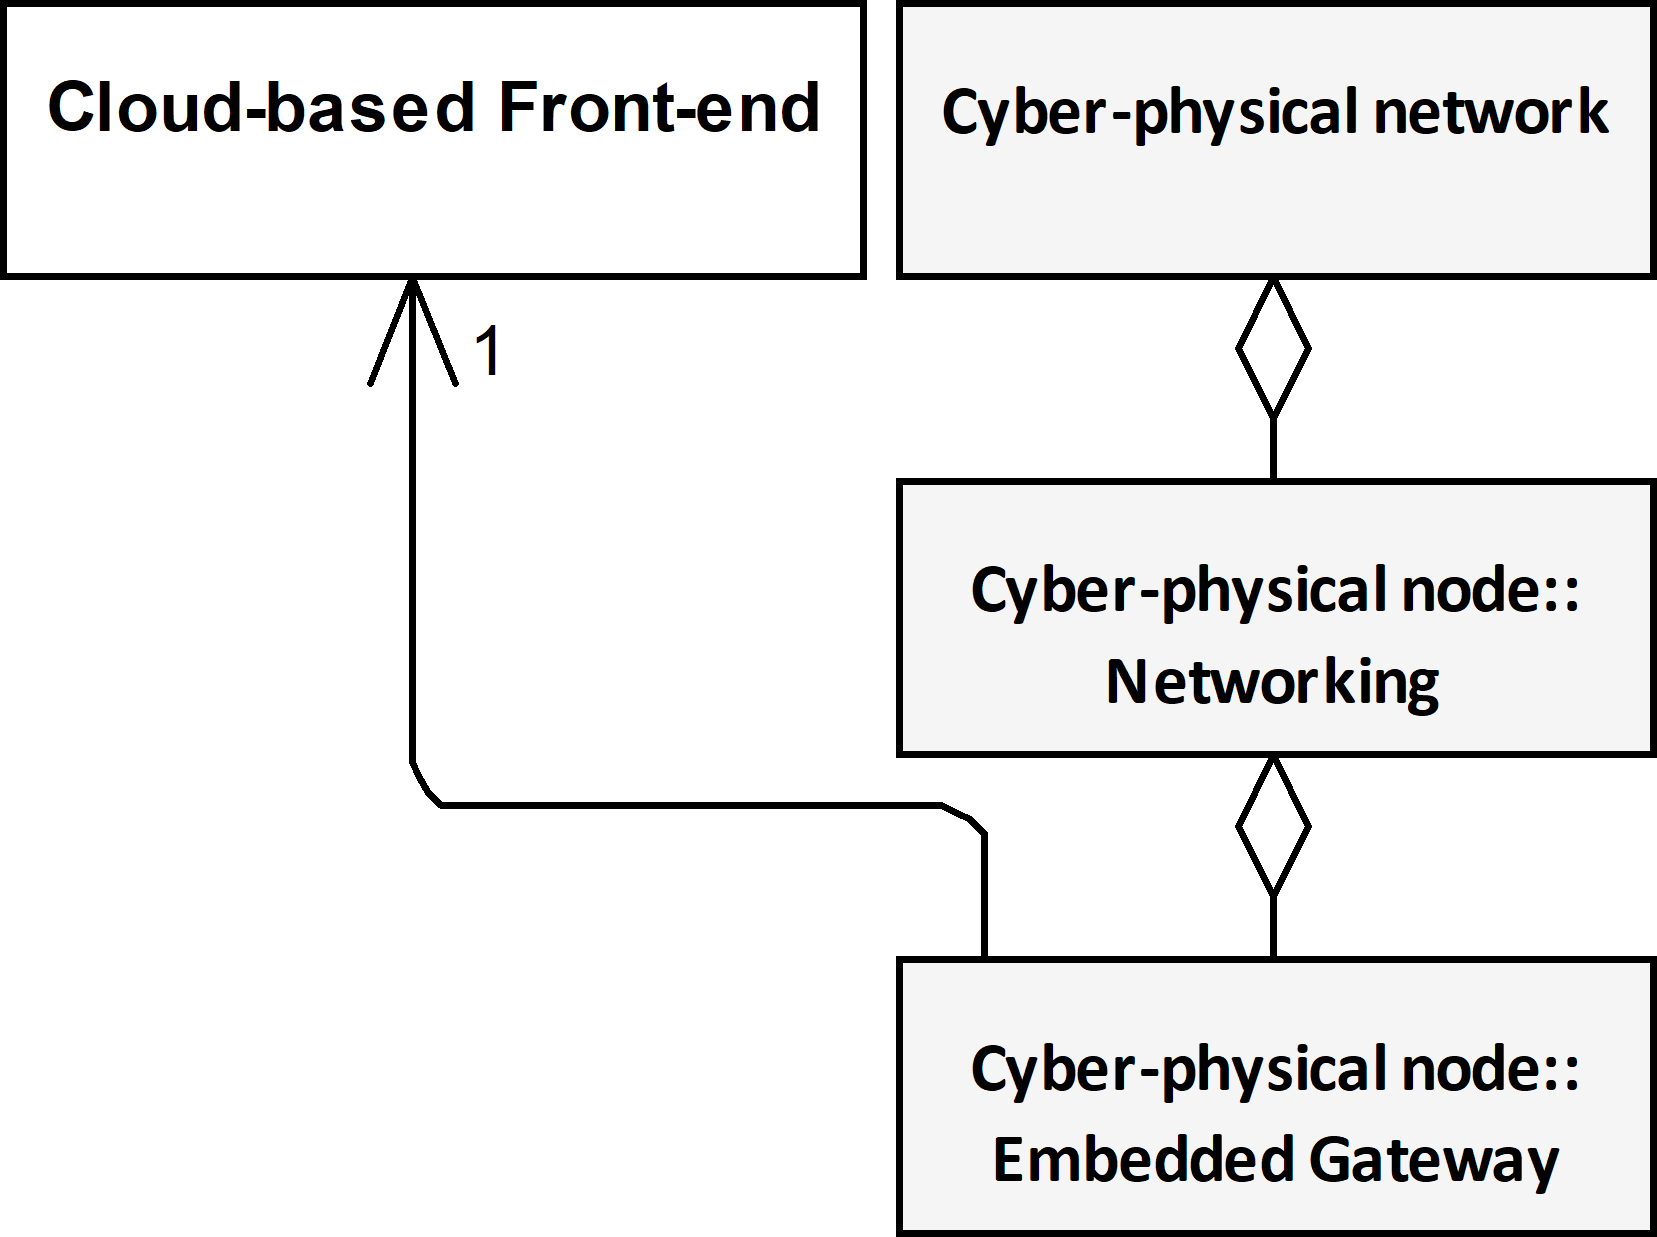
\includegraphics{../.Media/StrategyDomainModel.png}
  \caption{Strategy Domain Model}\label{StrategyDomainModel}
\end{figure}

Unlike the above described solutions, the \textbf{embedded gateway} is
not derived from the middleware concept. The domain model for this
archetype is presented in the Fig.~\ref*{StrategyDomainModel} Promoting separation of concern
design principle, the gateway functionality should be implemented as a
self-contained software part embedded in the \texttt{Networking} service
of the \texttt{Cyber-physical\ node}. Main functionality of this
component is to transfer selected data between
\texttt{Cyber-physical\ network} using \texttt{Networking} services of
an existing \texttt{Cyber-physical\ node} and
\texttt{Cloud-based\ front-end} using officially supported by the cloud
vendor interconnection services.

The \textbf{embedded gateway} archetype relaxes most of the issues
described above: \texttt{Cyber-physical\ network} real-time behavior, data
encoding incompatibility, security-context differences to name only a
few. The main goal of this article is to provide proof that the
\textbf{embedded gateway} archetype implementation is possible based on
a generic architecture that can be used as a foundation for the
integration of the heterogenous environments in concern. The proposed
implementation is designed for selected interoperability standard and
cloud product.

To comply with the Industry 4.0 communication criterion it is required that any product must be addressable over the network via TCP/UDP or IP and has to support the OPC UA Information Model. As a result, any product being advertised as Industry 4.0 enabled must be OPC UA-capable somehow. To support the multi-vendor environment OPC Unified Architecture interoperability standard has been selected. OPC UA supports the following two patterns to be used to transfer data between communicating parties:

\begin{itemize}
  \tightlist
  \item \textbf{session-oriented}: requires a session that has to be established before any data can be sent between sender and receiver
  \item \textbf{sessionless-oriented}: the sender may start sending messages (called packets or datagrams) to the destination without any preceding handshake procedure
\end{itemize}

Using the session-oriented communication pattern it is difficult or
even impossible to gather and process mobile data (Sec. I), which is one
of the Internet of Things paradigms. OPC UA Part 14 PubSub \cite*{RefWorks:doc:5d98837de4b055984c0eecf0} \todo{add ref: Mariusz Postol, UA Part 14: PubSub Main Technology Features in Object Oriented Internet, https://github.com/mpostol/OPC-UA-OOI, 2019, DOI: 10.5281/zenodo.1198852} offers the sessionless approach as an additional option to session based client-server interoperability relationship and is a consistent part of the OPC UA specifications suit. As the result it can be recognized as the IoT ready technology.

The presented proposals in the article are backed by proof of concept
reference implementations. For this study, prototyping addresses
Microsoft Azure cloud products. There are many reasons for selecting
Azure to accomplish cloud-based front-end of Cyber-Physical System (CFS). Azure offers
Infrastructure as a Service (IaaS) and Platform as a Service (PaaS)
capabilities. As a result, the platform can be used not only as a
cloud-based front-end for CFS. By design, the Azure services are
compliant with Security Development Lifecycle (SDL) an industry-leading
security process. It is also compliant with the new international
standard for cloud privacy, namely ISO 27018. Solutions hosted on Azure
are scaled up to millions of users without any additional coding. For
the development of the CFS front-end, it is essential that Azure
provides very efficient storage services usefully for real-time process
data archival. Azure provides a vast variety of hybrid connections
including but not limited to virtual private networks (VPNs), caches,
content delivery networks (CDNs), ExpressRoute, and IoT dedicated
services that can be directly used to implement cloud-based front-end
for CFS. Because it is also integrated with other Microsoft tools like
Office 365, Outlook, and SharePoint using Azure allows preserving
investment and exporting process data to the mentioned tools. Azure also
offers services supporting analytics and intelligence capabilities for
further improving business processes and decision making. It is the only
cloud platform that offers Blockchain as a Service (BaaS), Machine
Learning, Bots, and Cognitive APIs capabilities.

Azure aids Internet protocols and open standards such as JSON, XML,
SOAP, REST, MQTT, AMQP, and HTTP. A software development kits for C\#,
Java, PHP, and Ruby are available for custom applications. Azure
provides services supporting data exchange over the OPC UA, but they
don't support pubsub compliant with the OPC UA Part-14. Connectivity
services on the network use JSON-based Data Transfer Object encoded
based on schema derived from the solution metadata.

More detailed description of the selected Azure features in context of the application in concern are covered by the Sec.~\ref*{azure-main-technology-features}.

Based on the sessionless and session-oriented communication patterns examination against the IoT requirements \cite{mpostol2020} it could be concluded that the connectionless pattern better suites issues related to the assets mobility and traffic asymmetry that is characteristic for the application domains in concern. Additionally, to promote
interoperability and address the demands of the M2M communication in the context of a multi-vendor environment the prototyping should use an
framework that must be compliant with the OPC UA Part 14 PubSub spec \cite{RefWorks:doc:5d98837de4b055984c0eecf0}. According to proposed architecture presented in Fig.~\ref*{StrategyDomainModel} to implement the \texttt{Embedded\ Gateway} as a composable part of the \texttt{Cyber-physical\ Node} a library implementing \texttt{Networking} functionality in compliance with mentioned above specification is a starting point for further development. Additionally it must be assumed that the library used to deploy \texttt{Embedded\ Gateway} support dependency injection and be capable to compose an external part supporting Azure/pubsub gateway functionality. The composition process must be available without modification of the core code of an existing library. As a result the prototyping is to be limited to implementation of the \texttt{Embedded\ Gateway} software part only.

A library that meets all these requirements has been implemented consistently with the Object-Oriented Internet paradigm \cite{RefWorks:doc:5c66740ae4b081adf5804596}
worked out in an open-source project \footnote{ \url{https://github.com/mpostol/OPC-UA-OOI} }. The \cite{mpostol2020}
covers the description of a reference application program implementation proving that it is possible to design
universal architecture targeting reactive interoperability as a
consistent part of the Object-Oriented Internet concept compliant with
the OPC UA PubSub \cite{RefWorks:doc:5d98837de4b055984c0eecf0} international standard. According to the presented implementation and
evaluation, using the dependency injection and late binding, the
application program can be seamlessly adapted to the production
environment and scales well. This approach also improves flexibility and
adaptability of the existing solutions against any modification of the
production environment including but not limited to the selected
interoperability standard change.

Sect.~\ref*{ooi-main-technology-features} provides more detailed description of this library and part deployment process to implement new functionality supporting (\texttt{Embedded\ Gateway}.

The following subsections covers description of the current state of technologies with regards to OPC UA pubsub and Azure cloud-based IoT enabler.

\hypertarget{azure-main-technology-features}{%
  \subsection{Azure Main Technology Features}\label{azure-main-technology-features}}

\hypertarget{services}{%
  \subsubsection{Services}\label{services}}

Deployment of the hybrid solution providing interoperability of the
\textbf{machine-centric} cyber-physical systems designed atop of M2M
reactive communication and emerging cloud computing as a
\textbf{human-centric} front-end requires decisions addressing the
selection of the services supporting web user interface capable to
expose process data. In this context, the service is any
autonomous (with own identity) software component or module that is
interfacing with selected cyber-physical systems for data collection,
analysis, and also remote control. Microsoft Azure is a cloud-based
product. It offers a vast variety of services. This virtual environment
handles an unlimited number of users and devices organized using a
solution concept. The solution aggregates users, devices, services, and
required additional resources scoping on a selected scenario. The
solution serves as a context that provides a scope to the identifiers
(the names of devices, users, process data entities, etc) inside it.
Solutions are used to organize deployment entities into logical groups
and prevent identity collisions.

The \texttt{IoT\ Central} service provides a process data visualization
user interface. To make this interface meaningful metadata called device
template is used to describe devices.

Following the assumption that interconnection between the cyber-physical
system and cloud services is designed based on the gateway concept, a
middleware must be considered as a coupler. It must be interconnected
with the cyber-physical system using an in-band protocol adhering to
communications requirements (i.e.~protocol profile, data encoding, time
relationships, etc.) governing communication of the parts making it up.
At the same time, it must support back-and-forth data transfer to the
cloud using out-of-band native for the cloud services. The transfer
process requires data conversion from source to destination encoding.
The \texttt{IoT\ Hub} is a service hosted in the cloud that supports
\texttt{IoT\ Central} providing a robust messaging solution - it acts as
a central message hub for bi-directional communication. This
communication is transparent, i.e.~it is not data types aware allowing
any devices to exchange any kind of data. This service is responsible to
manage the devices' identity and it offers the following protocol
stacks: AMQP, MQTT, HTTPS.

Before process data can be exposed using a web user interface the data
source must be associated with an appropriate solution and validated to
make sure that the security rules are not violated. It is hard to assume
that the security rules governing the cyber-physical system may also
apply to the cloud-based services. In the gateway scenario, they can be
mapped on each other or entirely independent. The
\texttt{IoT\ Hub\ Device\ Provisioning\ Service} (DPS) is a helper
service for \texttt{IoT\ Hub} that enables devices' connection process
management, upon device providing valid identity attestation it assigns
the device to an appropriate \texttt{IoT\ Hub} instance and returns to
the device connection parameters, which allow direct connection with
given \texttt{IoT\ Hub} service. The device proceeds to use the same
attestation in \texttt{IoT\ Hub} connection and based on it, is granted
authorization to selected resources \todo{MP authorization can be applied only to operations?} and operations including but not limited to data transfer updating the user interface.

It is worth stressing that interaction of the offered by the Azure
services can be configured flexibly, and as a result, the presented
above selection of services must be recognized as an example only. The
\texttt{IoT\ Central} can be also seamlessly integrated with other
services as needed. The following services could also be considered to
build cloud-based automation solution:

\begin{itemize}
  \tightlist
  \item
        \texttt{Industrial\ IoT} - discovering OPC UA enabled servers in a factory network and register them in Azure \texttt{IoT\ Hub} implemented using \texttt{IoT\ Edge}
  \item
        \texttt{Digital\ Twins} - managing the graph of digital twins, which are to represent some real-world process or entity
\end{itemize}

\texttt{Industrial\ IoT} promotes OPC UA client/server archetype used to
achieve direct and interactive interoperability implemented using
\texttt{IoT\ Edge} services that allow extracting initial data
processing to local premises based on the edge concept.
\texttt{Digital\ Twins} is an emerging concept to use an observer to
replicate selected process state and behavior. The possibility to add
value as a result of using these services must be subject to further
research.

\hypertarget{data-interchange}{%
  \subsubsection{Data Interchange}\label{data-interchange}}

System components interoperability means the necessity of the
information exchange between them. The main challenge of
interoperability implementation is that information is abstract -- it is
knowledge describing the process in concern state and behavior,
e.g.~temperature in a boiler, a car speed, an account balance, etc.
Obviously, abstraction cannot be processed by the cyber-physical
machines. It is also impossible to transfer abstraction from one place
to another over the network.

Fortunately, computer science offers a workaround to address that
impossibility - the information must be represented as a binary stream.
In consequence, we can usually use both ones as interchangeable terms
while talking about ICT systems. Unfortunately, these terms must be
precisely observed in the context of further discussion, because we must
be aware of the fact that the same information could have many different
but equivalent representations. In other words, the same information can
be represented by a vast variety of different binary patterns. For
example, numbers may be represented using 2's Complement and
Floating-Point binary representations.

It should be nothing new for us, as it is obvious that the same
information printed as a text in regional newspapers in English, German,
Polish, etc. does not resemble one another, but the text meaning should
always be the same. To understand a newspaper we must learn the
appropriate language. To understand the binary data we must have defined
a data type -- a description of how to create an appropriate bits
pattern (syntax) and rules needed to assign the information (semantics),
i.e.~make any correct bitstream meaningful. Concluding, to make two
systems interoperable, a semantic-context must be established. The type
plays the role of metadata, a set of data that describes other data.
Metadata term is frequently used if the semantic-context is defined
using a native language to select built-in types engaging a
general-purpose graphical user interface.

Using the data type definitions to describe information interchanged
between communicating parties allows:

\begin{itemize}
  \tightlist
  \item
        Development against a type definition of the user interface
  \item
        Implementation of the functionality of the bitstreams conversion in
        advance
\end{itemize}

Having defined types in advance, a gateway may provide dedicated conversions functionality, i.e.~replacing bitstreams used by the cyber-physical system by equivalent ones for the cloud-based services. The Azure offers a vast variety of built-in types ready to be used in common cases, but not necessarily there are equivalent counterparts in use by the cyber-physical system. Additionally, the data conversion must address the following issues:

\begin{itemize}
  \tightlist
  \item
        usually to covert data from source to destination representation, the
        middleware software native types must be used
  \item
        if the out of the box set of types is not capable of fulfilling more
        demanding needs, custom data types must be defined
\end{itemize}

Although the data conversion is a run-time gateway task the
implementation of the conversion algorithms must be recognized as an
engineering task, and therefore this topic is not considered for further
discussion.

In \texttt{IoT\ Central} a cyber-physical system is represented as a set
of devices. The characteristics and behavior of each device kind are
described by the device template. This Device Template (DT) contains
also metadata describing the data (called telemetry) exchanged over the
wire with the cyber-physical system called Device Capability Model
(DCM). Additionally, the DT contains properties, customization, and
views definitions used by the service locally. As an option, DCM
expressed as a JSON-LD can be imported into a Device Template.
\texttt{IoT\ Central} allows also to create and edit a DCM using the
dedicated web UI. A JSON file containing DCM can be derived from an
information model used as a foundation to establish the semantic-context
applied to achieve interoperability of the devices interconnected as the
cyber-physical system. DCM development against any external information
model is a design-time task and should be supported by dedicated
development tools. In any case, the data interchanged between the cloud
and the gateway must be compliant with the DCM, hence the middleware
software must be aware of conversions that must be applied to achieve
this interoperability.

\hypertarget{connectivity}{%
  \subsubsection{Connectivity}\label{connectivity}}

From the cloud side, it is proposed to employ the \texttt{IoT\ Hub}
service to handle the network traffic targeting the cyber-physical
system. This service offers profiles of the AMQP, MQTT, HTTPS protocol
stacks. In any case, process data (telemetry) is transparently
transferred back-and-forth to the upper layer \texttt{IoT\ Central}
service. Hence, the payload formatting is determined by the DCM
associated with the \texttt{IoT\ Central} solution. All the mentioned
protocols are standard ones. Consequently, it is possible to apply any
available implementation compliant with an appropriate specification to
achieve connectivity. In this case, all parameters required to establish
connectivity and security-context is up to the external software
responsibility. Alternatively, the API offered by the dedicated
libraries may be used. Using this API the configuration process can be
reduced significantly. Using these libraries, the selection of the
communication protocol has an indirect impact on the interoperability
features, including performance. The connectivity with
\texttt{IoT\ Hub}, for example, can be obtained using:

\begin{itemize}
  \tightlist
  \item
        \texttt{Microsoft.Azure.Devices} - Service SDK for Azure IoT Devices
  \item
        \texttt{Microsoft.Azure.Devices.Client}- Device SDK for Azure \texttt{IoT\ Hub}
  \item
        \texttt{Microsoft.Azure.Devices.Shared} - Common code for Azure IoT
        Device and Service SDKs
  \item
        \texttt{Microsoft.Azure.Devices.Provisioning.Client} - Provisioning
        Device Client SDK for Azure IoT Devices
  \item
        \texttt{Microsoft.Azure.Devices.Provisioning.Transport.Amqp} -
        Provisioning Device Client AMQP Transport for Azure IoT Devices
  \item
        \texttt{Microsoft.Azure.Devices.Provisioning.Transport.Http} -
        Provisioning Device Client Http Transport for Azure IoT Devices
  \item
        \texttt{Microsoft.Azure.Devices.Provisioning.Transport.Mqtt} -
        Provisioning Device Client MQTT Transport for Azure IoT Devices
\end{itemize}

\hypertarget{ooi-main-technology-features}{%
  \subsection{OOI Main Technology Features}\label{ooi-main-technology-features}}

\begin{itemize}
  \tightlist
  \item
        Machinie To Machine communication based on the semantic data
  \item
        OOI PubSub Implementation Architecture
  \item
        Simple, complex and structural data processing
\end{itemize}


\hypertarget{gateway-implementation}{%
  \section{Azure - Object-Oriented Internet interoperability Implementation}\label{gateway-implementation}}

\begin{itemize}
  \tightlist
  \item
        Architecture
  \item
        Protocol selection and mapping
  \item
        Configuration
  \item
        Testing
\end{itemize}

\hypertarget{conclusion}{%
  \section{Conclusion}\label{conclusion}}

The OPC UA PubSub to Azure gateway (\texttt{AzureGateway})
implementation has been just published on GitHub as the open-source (MIT
licensed) as a part of the more general concept of the Object-Oriented
Internet reactive networking. It is proof of the concept that

\begin{enumerate}
  \def\labelenumi{\arabic{enumi}.}
  \tightlist
  \item
        OPC UA PubSub can be implemented as a powerful standalone package - no C/S dependency
  \item
        Azure interoperability can be implemented as an out-of-band
        communication (MQTT, AMQP, HTTP) - no PubSub dependency
  \item
        Process data functionality can be composable at run-time - no
        programming required
\end{enumerate}

\bibliography{Manuscript.bib}
\bibliographystyle{aiaa-jacs.bst}

\end{document}
